\chapter{Entorno de desarrollo}

Este capítulo describe el proceso seguido para establecer el entorno de desarrollo, incluyendo los problemas que se encontraron, las soluciones que se tomaron y finalmente el resultado obtenido. Este entorno servirá de base para el trabajo posterior en los siguientes capítulos que, como está descrito en la sección de condiciones de diseño, tiene como función principal habilitar la validación del trabajo realizado por medio de la técnica ``Processor-in-Loop''.

\section{Selección de autopiloto base}

Existe un requisito que inmediatamente acota la selección de autopiloto, el software debe ser de código abierto debido a que posiblemente el código se deba modificar en caso de que las opciones de configuración del autopiloto no sean suficientes para cumplir los objetivos. En el laboratorio de técnicas aeroespaciales se cuenta con hardware Pixhawk programado con el firmware de fábrica PX4.

\begin{figure}[h]
    \centering
    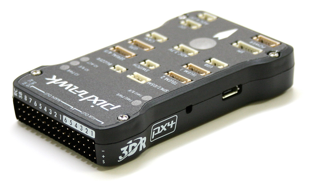
\includegraphics{hardware-pixhawk.png}
    \caption{Autopiloto Pixhawk}
    \label{fig:pixhawk1}
\end{figure}

El hardware autopiloto Pixhawk se puede programar con otro software distinto al del fabricante, entre aquellas soluciones las que son aplicables y de código abierto son ArduPilot, iNAV y Paparazzi, además de PX4 que también cumple con las condiciones de diseño \cite{survey}. iNAV no ofrece opciones de vuelo autónomo avanzadas como aterrizaje automático, que serán de interés en el capítulo de diseño de algoritmos de control. Paparazzi es una opción bastante interesante que si tiene un sistema autónomo completo por medio de archivos ``XML'' con la información del plan de vuelo \cite{paparazzi_flight_plan}, pero no es compatible con el software de control en tierra utilizado por ArduPilot y PX4, siendo Mission Planner y QGroundControl los principales.

\begin{figure}[h]
    \centering
    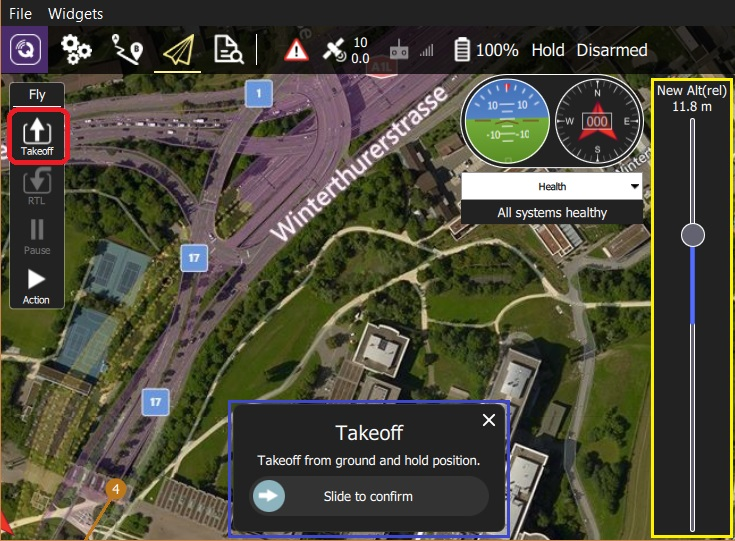
\includegraphics[width=0.7\textwidth]{takeoff.jpg}
    \caption{Software de estación en tierra QGroundControl}
    \label{fig:qgroundcontrol}
\end{figure}

PX4 es una opción atractiva ya que ofrece soporte para trabajar con técnicas ``Hardware-in-the-Loop'' con simuladores incluyendo X-Plane \cite{px4-hitl}. Sin embargo, aunque ArduPilot haya deprecado esa opción \cite{ap-hitl} existe más documentación en comparación con PX4 sobre como modificar existentes e implementar nuevos algoritmos de control \cite{ap-custom-controller}. Por esto último se decide en ArduPilot como plataforma de desarrollo.

y será provechoso si ya existen esfuerzos por agregar la capacidad de algoritmos personalizados a alguno de estos lo que reduciría trabajo. Una solución que se acerca a esta visión es la de recompilar ArduPilot junto con código exportado de Simulink para la implementación de nuevos controladores \cite{ardupilot-custom}.

\section{Extensión de protocolo de comunicación}
